\documentclass{article}
\usepackage{arxiv}


\title{A conditional permutation-based approach to test confounder effect and center-bias in machine learning models}


\author{
  Tamas~Spisak \\
  Institute for Diagnostic and Interventional Radiology and Neuroradiology \\
  University Hospital Essen\\
  Hufelandstrasse 55, 45147 Essen \\
  \texttt{tamas.spisak@uk-essen.de} \\
  %% examples of more authors
  %% \AND
  %% Coauthor \\
  %% Affiliation \\
  %% Address \\
  %% \texttt{email} \\
  %% \And
  %% Coauthor \\
  %% Affiliation \\
  %% Address \\
  %% \texttt{email} \\
  %% \And
  %% Coauthor \\
  %% Affiliation \\
  %% Address \\
  %% \texttt{email} \\
}

\begin{document}
\maketitle

\begin{abstract} % 150 words
\lipsum[1]
\emph{'mlconfound'}\footnote{https://github.com/pni-lab/mlconfound}
\end{abstract}


% keywords can be removed
\keywords{machine learning, predictive modelling, confounder, conditional independence test, conditional permutation test}

%%%%%%%%%%%%%%%%%%%%%%%%%%%%%%%%%%%%%%%%%%%%%%%%%%%%%%%%%%%%%%%%%%%%%%%%%%%
\section{Introduction}

Predictive modelling and supervised learning methods have recently became increasingly important in biomedical research and hold promise for delivering biomarkers that substantially impact clinical practice and public health \citep{kent2018personalized}. The usefulness and applicability of the such markers is to be evaluated not solely on the biomedical relevance of the predictive performance (i.e. prognostic/diagnostic value); generalizability across contexts and populations and biomedical validity (i.e. the model is driven by biomedical relevant signal) are also highly important requirements towards potential biomarkers \citep{woo2017building}.

Variables that can induce spurious associations between the predictor variables (features) and the prediction target - often referred to as confounders - can be detrimental to the model's biomedical validity and generalizability. Many types of confounders can be distinguished.
First, measurement artifacts can obviously be considered as confounders. For instance, in-scanner head motion artifacts in magnetic resonance imaging (MRI)-based predictive models can be especially problematic, if the prediction target is also associated with movement kinematics or motor function, like previously demonstrated e.g. in case of e.g Autism \citep{spisak2014voxel, spisak2019optimal} and Alzheimer's \citep{rao2017predictive}. Similarly, eye-blink artifacts can result in confound-bias in EEG-based markers \citep{eldridge2014robust}.
Second, depending on the research question, demographic and psychometric variables can also be considered as confounders during predictive modelling. E.g. resting-state functional connectivity is known to be strongly predictive to  demographic age \citep{wang2012decoding, dukart2011age} and moderately to fluid intelligence \citep{he2020deep, cole2012global}. As fluid intelligence is known to decline with aging, \citep{kievit2018neural}, models trained to predict intelligence can provide reasonable performance by simply picking up on age-related variance. 
Third, center-effects (or in general, batch effect) in multi-center studies can also cause significant bias in predictive models \citep{leek2010tackling, da2020performance}. In this case, predictive models can utilize center-effects to explain (random or true) center-differences in the predictive target. Such models will display worse-than-expected performance when applied on data from new centers.

Recently, various data harmonization approaches have been suggested to mitigate confounder-bias, ranging from simple matching \citep{rao2017predictive} or regression-based techniques \citep{rao2017predictive, dukart2011age, spisak2014voxel, abdulkadir2014reduction} to the popular non-parametric empirical Bayes-based method of \cite{johnson2007adjusting} or sophisticated deep-learning oriented solutions \citep{zhao2020training, hognon2019standardization}). However, it is often unclear which variables should be considered as confounders during harmonization and considering many variables as confounder holds risks of eliminating signal-of-interest \citep{wachinger2021detect}.

Powerful statistical tests to quantify the confounding effect of certain variables in predictive models could largely foster both the the identification of confounders to correct for and the assessment of the effectiveness of various harmonization or other confound-mitigation approaches. Such methods, however, have to tackle the fact that the outputs of predictive models often have non-normal distributions (due to e.g. regularization) \citep{garcia2009study, kristensen2017whole}.

Recently three dedicated techniques \citep{chaibub2019permutation, ferrari2020measuring, wachinger2021detect} have been proposed for quantifying confounder bias in predictive modelling.

The permutation-based approach of \cite{chaibub2019permutation} evaluates the null-hypothesis of no confounder bias via restricted permutations. It's p-values, however, might be invalid in certain circumstances (e.g. biased classification problems) and, as shown by \cite{ferrari2020measuring}, it does not guarantee a proper type I error control.
The 'confounder index' (CI) proposed by \cite{ferrari2020measuring}, by design, does not provide any quantification of statistical significance.
Moreover, both approaches involve repeated re-fitting of the machine learning model, which might not be feasible for models with high computational complexity (especially when hyperparameters are optimized in a nested cross-validation).
The Kolmogorov Complexity-based causal inference test, as proposed by \cite{wachinger2021detect}, aims at determining whether it is more likely that the the predictor(s) are a direct cause of the target variable or, alternatively, there exists an unobserved random variable that is the cause of both. It's computation assumes 'faithfulness' (if two variables are independent, there is no direct influence between the two in the underlying graph) a strong condition that might not be fulfilled in many real applications (e.g. functional MRI is an \emph{indirect} measure of neural activation, rendering the alternative hypothesis true in absence of any real confounder).

% todo: RO and CI: classification, KC: regression

In this paper, I formulate the 'confounder problem' as a special case of conditional independence testing \citep{dawid1979conditional}. This allows relating the problem to the seminal work of \cite{shah2020hardness}, who showed that, without placing some assumptions on the joint distribution of the involved variables, establishing a conditional independence test with a valid type I error control and non-trivial power is effectively impossible ("no free lunch" theorem).

Next, I consider the conditional permutation test, a statistical test of conditional independence, recently introduced by \cite{berrett2020conditional}, as a test for evaluating confounder-bias of predictive models.

Within this framework, various confounder-related null hypotheses can be tested, so that no assumption is to be made about the distribution of one of the conditioned variables. As normality is typically a reasonable assumption for the target and confounder variables but not for the predictions of the model, the focus is put on the cases allowing inference without assumptions on the model predictions' distribution.
Two cases satisfy this requirement, one testing whether the model's explained variance can be exclusively attributed to the confounder and the other testing whether the model utilizes any confounder-variance, above what's already present in the target variable.
Both tests require only on the target variable, the model predictions and the putative confounder, that is, they can be performed without needing to re-fit the model.
Additionally, a regression-based estimation of the conditional distribution of $c|y$ is proposed, which allows testing confounder bias without a-priory knowledge about the conditional distribution and without any assumptions on the distribution of the predicted values (which are often non-normal in practice).
The validity of the type I error control and the statistical power of both tests are evaluated with simulated data (assuming non-normal model output).
The proposed tests are then applied on functional brain connectivity data to provide evidence of motion-bias in a model trained on the Autism Brain Imaging Data Exchange (ABIDE) dataset \citep{di2014autism} and to evaluate the age dependence of fluid intelligence predictions on data from the Human Connectome Project.




\begin{itemize}
    \item growing interest in the use of
supervised learning in biomedical contexts
    \item confounder effects, site-effects
    \item approaches to deal with confounders can
    \item these approaches can eliminate signal-of-interest
    \item need for an approach that can quantify the effect of a con- founding variable and assess the effectiveness of the possible counter- measures
    \item parametric methods might fail (regularization)
    \item current solutions:
    \begin{itemize}
        \item RP: invalid p-values, continuous only with binning, involves repeating whole model training
        \item CI: no p-value, continuous only with binning, involves the whole model training
    \end{itemize}
    \item proposed method:
    \begin{itemize}
        \item based solely on the target, confounder and prediction
        \item utilizes a mathematically established non-parametric framework for testing conditional independence of the confounder and the predictions, given the observed target
        \item i.e. testing the null hypothesis that the prediction does not capture more confound than what is already present in the target variable
        \item which is usually of primary interest when investigating confounder-bias of machine learning models.
    \end{itemize}
\end{itemize}

%%%%%%%%%%%%%%%%%%%%%%%%%%%%%%%%%%%%%%%%%%%%%%%%%%%%%%%%%%%%%%%%%%%%%%%%%%%
\section{Methods}

\subsection{Notation and Background}

In a predictive modelling setting, let $Y$ denote the target variable, $\hat{Y}$ denote model output, i.e. the predictions for $Y$ and let $C$ denote a variable, which is considered as a confounder. Depending on the research question, the influence of $C$ on the model predictions $\hat{Y}$ is subject to be kept at a negligible level, or it is to be proven that the model is not completely driven by $C$. Below, I summarize how testing conditional independence \citep{dawid1979conditional} among these variables allows addressing the above questions and build on the conditional permutation test of \cite{berrett2020conditional} to perform inference without assumptions on the distribution of the model output, where normality is often violated \citep{garcia2009study, kristensen2017whole}.

\subsubsection*{Testing conditional independence}

Let us shall assume that the data consist of independent and identically distributed (IID) data points $(x_i, y_i, z_i) \in X \times Y \times Z$ for $i=1, \dots , n$ and write $X=(x_1, \dots ,x_n)$, $Y=(y_1, \dots, y_n)$ and $Z=(Z_1, \dots, Zn)$. 

$X$ is \emph{conditionally independent} of $Y$ given $Z$ $X \independent Y | Z$, if for all $x, y, z$ with $p(z) > 0$, we have $p(x, y|z) = p(x|z)p(y|z)$ \citep{dawid1979conditional}.

While conditional independence lies at the heart of several fundamental concepts is statistics and  plays an increasingly important role in various fields of applied statistics (and particularly in biomedical applications, \citep{spirtes2000causation, peters2016causal, fiedler2011mediation, candes2016panning}, recently, \cite{shah2020hardness} have raised important concerns regarding conditional independence testing.
In their "no free luch" theorem, Shah and Peters has shown that, without placing some assumptions on the joint distribution of $(X, Y, Z)$, conditional testing is effectively impossible. In other words, no test exists that - for all distributions - provides a valid type I error control and, at the same time, has a non-trivial statistical power.

This result is in strong contrast to unconditional independence testing, for which permutation tests  \citep{pitman1937significance, fisher1942189} allow for the correct calibration of any hypothesis test. Even if the null hypothesis $H0 :X \independent Y|Z$ is true, $X$ and $Y$ might be highly marginally dependent due to their dependence on $Z$,  thus the permutation null-distribution will be invalid.

The "no-free-lunch" theorem has important implications for confound-testing in predictive modelling where the distribution of the model outputs - depending on the applied machine learning model - is \emph{unknown}.

Nevertheless, as shown by \cite{berrett2020conditional}, if information about the conditional distribution $Q(X|Z)$ is available, sampling from a non-uniform distribution over the set of possible permutations $\pi$ can incorporate available distributional information into permutation-based inference and achieve a valid type I error control and a non-trivial power.
Below we give a short description of the procedure of \cite{berrett2020conditional}.

\subsubsection*{The conditional permutation test for independence}

The conditional permutation test (CPT) of \cite{berrett2020conditional} build on the conditional randomization test of \cite{candes2016panning} and ensures that \emph{no assumptions} are made about the distribution of the response variable Y but, instead, it is assumed that the conditional distribution of X given Z is known.

CPT generates a null-distribution for an arbitrary predefined test statistic $T(X,Y,Z)$ by sampling permutation based "copies" of $X$,

$$x_i^{(j)} \sim Q(\cdot|z_i) \ $$

where, $Q(.|z)$ denotes the conditional distribution of $X$ given $Z=z$ and $j=1,\dots, m$ indexes the copies of $X$ and so that so that $X^{(i)} = (x_1^{(j)}, \dots, x_n^{(j)})$ is a permutation of the original vector $X = (x_1, \dots, x_n)$. This mechanism creates copies $X^{(1)}, \dots ,X^{(m)}$ that are exchangeable with the original vector X under the null hypothesis that $X \independent Y | Z$.

Under the null hypothesis, the triples $(X,Y,Z), (X^{(1)},Y,Z),\dots,(X^{(m)},Y,Z)$ are all identically distributed and exchangeable, and so are the 
$$T(X,Y,Z), T(X^{(1)},Y,Z),\dots,T(X^{(m)},Y,Z)$$
test statistics, as well.

The p-value under the null hypothesis is then obtained as
$$ p= 1+\frac{\sum_{j=1}^m \mathbb{1} \{T(X^{(j)},Y,Z) \geq T(X,Y,Z) \}  }{1+m}$$

Let $S_n$ denote the set of all permutations on the indices $\{1,\dots,n\}$ and $X_\pi = (x_{\pi_1}, \dots, x_{\pi_n})$ the vector $X$ with its elements reordered according to the permutation $\pi \in S_i$.
In the CPT procedure, the permutation-based copies of $X$ are consist of $x_i^{(j)} = x_{\pi^{(j)}}$ which are drawn so that 
so that:

\begin{equation}
    \mathbb{P}(\pi^{(j)} = \pi | X,Y,Z) = \frac{q^n(X_\pi | Z)}{\sum_{\pi' \in S_n} q^n(X_{\pi'} | Z)}
    \label{eq-pperm}
\end{equation}

that is, according to the $q^n(\cdot|Z) := q(\cdot | z_1, \dots q(\cdot|z_n)$ product density corresponding of the conditional distribution $Q(\cdot|z)$. Note that Eq. \ref{eq-pperm} does not necessarily assume a continuous distribution.
For a verification of the valid type I error control of this approach refer to Theorem 1 in \citep{berrett2020conditional}.

While the required permutations could be theoretically sampled with a simple Metropolis-Hastings algorithm that draws uniformly from $S_n$, at random, the acceptance ratio will be extremely low, even for moderate $n$ (except there is very low dependence of X on Z), resulting in slow mixing times. \cite{berrett2020conditional} (Algorithm 1) propose a parallelized pairwise Markov-Chain Monte Carlo sampler for CPT, that draws disjoint pairs in parallel and decides whether or not to swap them randomly, according to the odds ratio calculated from the conditional densities belonging to the original and swapped data. In their Theorem 2, \cite{berrett2020conditional} verify that the resulting Markov Chain yields the desired stationary distribution, even if the number of steps is small.

\subsection{Conditional Permutation-based confounder-bias test}

% fig:schematic
\begin{figure}
  \centering
  \resizebox{0.75\columnwidth}{!}{%
\tikzset{every picture/.style={line width=0.75pt}} %set default line width to 0.75pt        


\tikzset{every picture/.style={line width=0.75pt}} %set default line width to 0.75pt        

\begin{tikzpicture}[x=0.75pt,y=0.75pt,yscale=-1,xscale=1]
%uncomment if require: \path (0,300); %set diagram left start at 0, and has height of 300

%Shape: Circle [id:dp12907748114570317] 
\draw   (299.5,107) .. controls (299.5,93.19) and (310.69,82) .. (324.5,82) .. controls (338.31,82) and (349.5,93.19) .. (349.5,107) .. controls (349.5,120.81) and (338.31,132) .. (324.5,132) .. controls (310.69,132) and (299.5,120.81) .. (299.5,107) -- cycle ;
%Shape: Circle [id:dp12318976880062338] 
\draw   (397,39) .. controls (397,25.19) and (408.19,14) .. (422,14) .. controls (435.81,14) and (447,25.19) .. (447,39) .. controls (447,52.81) and (435.81,64) .. (422,64) .. controls (408.19,64) and (397,52.81) .. (397,39) -- cycle ;
%Shape: Circle [id:dp2655574667622329] 
\draw   (202,39) .. controls (202,25.19) and (213.19,14) .. (227,14) .. controls (240.81,14) and (252,25.19) .. (252,39) .. controls (252,52.81) and (240.81,64) .. (227,64) .. controls (213.19,64) and (202,52.81) .. (202,39) -- cycle ;
%Curve Lines [id:da9340239406716428] 
\draw    (250,28) .. controls (292,20) and (364,22) .. (400,28) ;
%Curve Lines [id:da6958426380393512] 
\draw    (239,61) .. controls (249,76) and (276,99) .. (299.5,107) ;
%Curve Lines [id:da8565840155201192] 
\draw    (349.5,107) .. controls (365,101) and (403,71) .. (410,60) ;

%Shape: Circle [id:dp9753164043561875] 
\draw   (475.5,257) .. controls (475.5,243.19) and (486.69,232) .. (500.5,232) .. controls (514.31,232) and (525.5,243.19) .. (525.5,257) .. controls (525.5,270.81) and (514.31,282) .. (500.5,282) .. controls (486.69,282) and (475.5,270.81) .. (475.5,257) -- cycle ;
%Shape: Circle [id:dp6395662810469516] 
\draw   (573,189) .. controls (573,175.19) and (584.19,164) .. (598,164) .. controls (611.81,164) and (623,175.19) .. (623,189) .. controls (623,202.81) and (611.81,214) .. (598,214) .. controls (584.19,214) and (573,202.81) .. (573,189) -- cycle ;
%Shape: Circle [id:dp786541411329625] 
\draw   (378,189) .. controls (378,175.19) and (389.19,164) .. (403,164) .. controls (416.81,164) and (428,175.19) .. (428,189) .. controls (428,202.81) and (416.81,214) .. (403,214) .. controls (389.19,214) and (378,202.81) .. (378,189) -- cycle ;
%Curve Lines [id:da22693900064180195] 
\draw    (426,178) .. controls (468,170) and (540,172) .. (576,178) ;
%Curve Lines [id:da6720989194231959] 
\draw    (415,211) .. controls (425,226) and (452,249) .. (475.5,257) ;
%Curve Lines [id:da8140666812849395] 
\draw    (525.5,257) .. controls (541,251) and (579,221) .. (586,210) ;
%Shape: Circle [id:dp471386481785639] 
\draw   (50,256) .. controls (50,242.19) and (61.19,231) .. (75,231) .. controls (88.81,231) and (100,242.19) .. (100,256) .. controls (100,269.81) and (88.81,281) .. (75,281) .. controls (61.19,281) and (50,269.81) .. (50,256) -- cycle ;
%Shape: Rectangle [id:dp8617145222488287] 
\draw   (156,237) -- (240,237) -- (240,277) -- (156,277) -- cycle ;
%Shape: Circle [id:dp8776576784951928] 
\draw   (290,256) .. controls (290,242.19) and (301.19,231) .. (315,231) .. controls (328.81,231) and (340,242.19) .. (340,256) .. controls (340,269.81) and (328.81,281) .. (315,281) .. controls (301.19,281) and (290,269.81) .. (290,256) -- cycle ;
%Shape: Circle [id:dp2868603849402189] 
\draw   (174,190) .. controls (174,176.19) and (185.19,165) .. (199,165) .. controls (212.81,165) and (224,176.19) .. (224,190) .. controls (224,203.81) and (212.81,215) .. (199,215) .. controls (185.19,215) and (174,203.81) .. (174,190) -- cycle ;
%Callout Right Arrow [id:dp26184503306970397] 
\draw   (46.55,225.27) -- (106,225.27) -- (106,250) -- (133,250) -- (133,241) -- (155.55,255.27) -- (133,269.55) -- (133,260.55) -- (106,260.55) -- (106,285.27) -- (46.55,285.27) -- cycle ;
%Right Arrow [id:dp7986276189609152] 
\draw   (240,250) -- (268,250) -- (268,241) -- (290,255.5) -- (268,270) -- (268,261) -- (240,261) -- cycle ;
%Shape: Circle [id:dp9535423837564185] 
\draw   (50,190) .. controls (50,176.19) and (61.19,165) .. (75,165) .. controls (88.81,165) and (100,176.19) .. (100,190) .. controls (100,203.81) and (88.81,215) .. (75,215) .. controls (61.19,215) and (50,203.81) .. (50,190) -- cycle ;
%Straight Lines [id:da6172567079022628] 
\draw    (75,215) -- (75,231) ;
%Straight Lines [id:da8731068989736062] 
\draw    (198,238) -- (198,215) ;

% Text Node
\draw (165,251) node [anchor=north west][inner sep=0.75pt]   [align=left] {ML model};
% Text Node
\draw (9,6) node [anchor=north west][inner sep=0.75pt]   [align=left] {\textbf{A}};
% Text Node
\draw (9,146) node [anchor=north west][inner sep=0.75pt]   [align=left] {\textbf{B}};
% Text Node
\draw (494,252.4) node [anchor=north west][inner sep=0.75pt]    {$C$};
% Text Node
\draw (591.5,180.4) node [anchor=north west][inner sep=0.75pt]    {$\hat{Y}$};
% Text Node
\draw (396,184.4) node [anchor=north west][inner sep=0.75pt]    {$Y$};
% Text Node
\draw (484,198) node [anchor=north west][inner sep=0.75pt]   [align=left] {CPT};
% Text Node
\draw (67,251.4) node [anchor=north west][inner sep=0.75pt]    {$X$};
% Text Node
\draw (308.5,247.4) node [anchor=north west][inner sep=0.75pt]    {$\hat{Y}$};
% Text Node
\draw (191,185.4) node [anchor=north west][inner sep=0.75pt]    {$Y$};
% Text Node
\draw (318,102.4) node [anchor=north west][inner sep=0.75pt]    {$Z$};
% Text Node
\draw (415.5,34.4) node [anchor=north west][inner sep=0.75pt]    {$Y$};
% Text Node
\draw (219,34.4) node [anchor=north west][inner sep=0.75pt]    {$X$};
% Text Node
\draw (308,48) node [anchor=north west][inner sep=0.75pt]   [align=left] {CPT};
% Text Node
\draw (68,185.4) node [anchor=north west][inner sep=0.75pt]    {$C$};


\end{tikzpicture}

    }
  \caption{Schematic diagram of using CPT in a predictive modelling context. \\ \textbf{(A)} CPT was originally proposed to be used on the feature variable $X$, target variable $Y$ and confounders $Z$. \textbf{(B)} The proposed use of CPT in predictive modelling requires the model to be fitted first, to obtain the model's prediction $\hat{Y}$ on $Y$. CPT is then utilized on the triplet $(Y, \hat{Y}, Z)$, to test hypotheses $\hat{y} \independent c | y$ or $y \independent \hat{y} | c$.}
  \label{fig:schematic}
\end{figure}

% tab:conditional-independence-cases
\renewcommand{\arraystretch}{2}
\begin{table}[]
\centering
\begin{tabular}{l|rp{60mm}|c|>{\centering\arraybackslash}m{30mm}}
 &  & H0  & assumption needed for: & no assumptions about the distribution of: \\
\hline
\textbf{1.} & $Y \independent \hat{Y} | C$ \quad  & model exclusively driven by confounder & $Q(\cdot|C)$ & $\hat{Y}$ or $Y$ \\
%\hline
\textbf{2.} & $Y \independent C | \hat{Y}$ \quad & model captures all variance in confounder & $Q(\cdot|\hat{Y})$ & $Y$ or $C$ \\
%\hline
\textbf{3.} & $\hat{Y} \independent C | Y$  \quad &  model does not capture more confound than what is present in the target & $Q(\cdot|Y)$ & $\hat{Y}$ or $C$ \\
\end{tabular}
\caption{\label{tab:conditional-independence-cases} Possibilities when testing conditional independence in potentially biased predictive models. \\The table lists the three possible null hypotheses (H0), and the variables where assumption about the joint/conditional distributions is required/not required.   ($Y$: prediction target, $\hat{Y}$: predictions, $C$: confounder variable) }
\end{table}

As many related papers, the work of \cite{berrett2020conditional} was formalized as a (semi-)supervised learning approach, where $X$ is the predictor(s) (features), $Y$ is the target variable and $Z$ is a potential confounder. In this setting, testing the null hypothesis $X \independent Y | Z$ aims to determine, whether $X$ affects $Y$, when controlling for $Z$.
For instance, in genome-wide association studies, CPT can be used o determine whether a particular genetic variant $X$ affects a response $Y$ such as disease status or some other phenotype, even after controlling for the rest of the genome, encoded in $Z$.

Here I consider a different setting, where supervised learning model is already fitted and we are focusing on model diagnostics, by testing the triplet $(Y,\hat{Y}, C)$, where $Y$ is the target variable, $\hat{Y}$ is the model's prediction for Y, an $C$ is the (possibly multivariate) confounder. In such a setting, we are interested in how much variance the fitted model captures from the confounder $C$ or, in other words, to what extent the model is biased by the confounder variable $C$ when predicting $Y$ with $\hat{Y}$. The conceptual difference between the original and the proposed application of CPT is depicted on Fig. \ref{fig:schematic}.

Conditional independence testing and, specifically, the framework of conditional permutation testing allows investigating three different null hypotheses corresponding to the $(Y, \hat{y}, C)$ triplet, as listed in Table \ref{tab:conditional-independence-cases}. Testing the null hypothesis $Y \independent \hat{Y} | C$ (option 1) investigates whether the model predictions are likely explainable solely with the confounder, i.e. whether the model is exclusively confounder-driven. Testing $Y \independent C | \hat{Y}$ (option 2) aims the question whether the model captures all the variance in $C$ when predicting $Y$. Testing the null hypothesis $\hat{Y} \independent C | Y$ (option 3) examines, whether the dependence of the model output on the confounder can likely be explained by the confounder's dependence on the target variable, i.e. whether there is any confounder bias in the model.

While option 3. is typically of interest when testing confounder bias of predictive models, option 1 might be also useful in diagnostics of predictive models, especially in the exploratory phase of model construction. Option 2 seems less appealing for model diagnostics and as detailed below, the proposed variety of the CPT framework does not allow forming a non-parametric method in this case.

Obtaining a relatively accurate, independent estimate of $D(\cdot|Z)$ (of any shape) for CPT inference is important. Berrett and colleagues recommend to use a large independent sample to obtain the log-likelihood matrix of the conditional distribution $D(\cdot|Z)$, which might be often viable in semi-supervised learning settings where unlabelled data $(X, Z)$ are easier to obtain than labelled data $(X, Y, Z)$.
Since in the proposed predictive modelling setting normality might be often a reasonable assumption for $Y$ and $C$ (but not for $\hat{Y}$), it is possible to fall back to Gaussian assumptions and thereby eliminate the need for a large, independent sample to estimate $D(\cdot|Z)$.

Here I propose to fit a linear regression model (or in case of categorical X, a logistic regression model):

\begin{equation}
    \label{eq:linreg}
    X = \alpha + \beta Z + \epsilon
\end{equation}


with the assumption that the residual error follows a Gaussian distribution and let $\mu = \alpha + \beta Z$ and $\sigma^2 = E(\epsilon^2)$. Then, for the conditional Normal distribution $ (X|Z=z) \sim \mathcal{N}\{\mu(z), \sigma^2(z)\}$ and the log-likelihood, that is to be used in Eq. \ref{eq-pperm}, can be computed as follows:

$$ \mathcal{L}(X|Z) = -{X^2}^T * \frac{1}{2} \sigma^2 + X^T \frac{\mu}{\sigma^2}$$

where $T$ means transposing row vectors to column vectors. 

Applying this Gaussian likelihood estimation in the case predictive model diagnostics requires that the two variables in Eq. \ref{eq:linreg} are substituted with $Y$ and $C$, but not $\hat{Y}$, for which the Gaussian assumption of the proposed likelihood estimation might not hold.

Therefore, from the three options for conditional independence-based null hypotheses, enumerated in Table \ref{tab:conditional-independence-cases}, this is possible for options 1 and 3, but not option 2, as the variable on which the independence is conditional must be always the predictor variable in Eq. \ref{eq:linreg}.

For options 1 and 3, the proposed simple Gaussian conditional likelihood estimation allows for deploying CPT without a large, independent sample to estimate the conditional distribution. 

---------------------------------


Todo: test statistic: $R^2$

The validity of the type I error control of CPT has been justified when using a true $D(\cdot|Z)$. While \cite{berrett2020conditional} gave bounds on the validity of the test given deviations from the true conditional distribution (which proved to be relatively tolerant against deviations from the true distribution), these bounds assume that the $D(\cdot|Z)$ has been estimated from an independent sample.

To provide foundations for the use of the proposed method we perfromed simulations...


-----------------------------

% tab:substitution
\renewcommand{\arraystretch}{2}
\begin{table}[]
\centering
\begin{tabular}{rl|l|l|l}
original & CPT & $X$ & $Y$ & $Z$ \\
\hline
%\hline
option 1: & full confounder test & $Y$ & $\hat{Y}$ & $C$ \\
%\hline
option 3: & partial confounder test & $C$ & $\hat{Y}$ & $Y$ \\
\end{tabular}
\caption{\label{tab:substitution} Substitutions of the symbols describing the variables in the original formulation of the CPT method and its two possible applications in predictive modelling diagnostics. }
\end{table}





%%%%%%%%%%%%%%%%%%%%%%%%%%%%%%%%%%%%%%%%%%%%%%%%%%%%%%%%%%%%%%%%%%%%%%%%%%%
\subsection{Validation on simulated data}

Using CPT to test confounder-bias in predictive modelling allows relaxing assumptions on $\hat{Y}$ (for both the partial and the full test) but - in line with the "no free lunch" theorem, requires knowing - or putting assumptions - on the joint distribution of the other two variables ($Y$ and $C$). 
\cite{berrett2020conditional} give a detailed analysis of the robustness of their CPT approach when estimating the conditional distribution with re-using the tested data and, also, against misspecifying the conditional distribution of interest.

Here I extend their results by performing validation that aids estimating the power of the test in a form that is accessible for power calculations in predictive modelling (considering various weights of the confounder and the target signals in $\hat{y}$ and in the case of varying levels of covariance between $Y$ and $C$).
Moreover, I perform a thorough investigation of the robustness of the test against the violation of normality (for both $(Y, C)$ and $\hat{Y}$).

Simulations are performed separately for the 'partial' and 'full' conditional confound tests.

\subsubsection*{Gaussian Simulations}
The target variable $Y$ and the confounder variable $C$ were drawn randomly from a multivariate normal distribution:

$$ Y, C \sim \mathcal{N}(\mu_0, \Sigma_\sigma) $$,

where $\mu=(0, 0)$ and the covariance matrix is given as:
$\Sigma_\sigma = \big(\begin{smallmatrix}
  1 & \sigma\\
  \sigma & 1
\end{smallmatrix}\big)$.

Next, we construct the simulated predicted values:

$$ \hat{Y} = w_Y Y + w_C C + w_e e$$

so that $w_Y + w_C + w_e = 1$, where $e \sim \mathcal{N}(0,1)$ is the noise component.

To test the implementation for categorical variables, simulated $Y$, $\hat{Y}$ and $C$ variables are binarized by thresholding at 0.

For more straightforward interpretation and visualization of the simulation results, the 'confound-to-target' and the 'signal-in-prediction' parameters were defined as

$$ w_{X/Y} = w_C / w_Y $$

and

$$ w_{C+Y} = w_C + w_Y $$,

respectively.

\subsubsection*{Introducing non-normality}

Non-normality is introduced by applying the \emph{sinh-arcsinh} transformation of \cite{jones2009sinh} on the simulated variables:

$$X' = sinh(\delta sinh^{-1}(X) - \epsilon)$$

where the parameters $\delta$ and $\epsilon$ control the kurtosis and skewness of the resulting \emph{sinh-arcsinh} distribution, with $\delta=1$ and $\epsilon=0$ producing the identity function (i.e. no non-normality introduced).

\subsubsection*{Simulation cases}

In the simulation procedure for the 'partial' confound test, 100 repetitions were performed of all combination of the following parameter values: 
\begin{itemize}
    \item covariance of $C$ and $Y$: $\sigma \in \{0, 0.2, 0.4, 0.6, 0.8\}$
    \item confound-to-target: $w_{C/Y} \in \{0, 0.1, 0.3, 0.5, 1\}$
    \item signal-in-prediction: $w_{C+Y} \in \{0, 0.3, 0.6, 0.9\}$
    \item sample size: $N \in \{50, 100, 500, 1000\}$
\end{itemize}

For testing 'full' confounder bias, identical parameters were used, except that instead of the 'confound-to-target' parameter $ w_{C/Y}$ we used the 'target-to-confound' parameter $ w_{Y/C} = w_Y / w_C $, but with the same parameter values $w_{Y/C} \in \{0, 0.1, 0.3, 0.5, 1\}$.

Next to the normally distributed case, 4 \emph{sinh-arcsinh} transformed cases were also investigated, with $\delta \in \{1, 1.05, 1.5, 5\}$ $\epsilon \in \{1, 3, 5, 10\}$ 

The 'partial' and 'full' confound tests, as implemented in version 0.7.1 of the package \emph{'mlconfound'} were run with default parameters, that is 1000 permutations and 50 Markov-chain Monte-Carlo steps to generate the conditioned permutations and by implying categorical variables, where needed.

Analysis code used for simulations is available\footnote{https://github.com/pni-lab/mlconfound/blob/master/validation/simulation.py} in the github repository of the 'mlconfound' package.

\subsection{Validation on functional brain connectivity data}

The usefulness of the proposed confounder tests is demonstrated by applying them for predictive classification and regression models based on functional brain connectivity data, with different confound-mitigation approaches. 

'Partial' and 'full' confound testing was used with default parameters (1000 permutations, 50 Markov-chain Monte Carlo steps) as implemented in version 0.7 of the package \emph{'mlconfound'}.

\subsubsection*{HCP: testing age- and acquisition batch-bias in fluid intelligence prediction}

Human Connectome Project contains imaging and behavioral data of more than 1000 healthy subjects \citep{van2013wu}. Preprocessed resting state fMRI connectivity data (partial correlation matrices) \citep{glasser2013minimal} as published with the HCP1200 release (N=999 participants with functional connectivity data) were used to build models that predict individual fluid intelligence scores (IQ), as measured with Penn Progressive Matrices \citep{duncan2000neural}.

To ensure normality, fluid intelligence scores were non-linearly transformed to normal distribution with the quantile transformation \citep{beasley2009rank} as implemented in \emph{scikit-learn} \citep{pedregosa2011scikit} (see Supplementary Figure \ref{fig:hcp-hist} for details).

Features (functional concavities across 100 group independent component analysis based regions) were either (i) considered in their raw form or were subject to confound mitigation approaches by (ii) feature regression \citep{rao2017predictive} or (iii) COMBAT \citep{johnson2007adjusting, fortin2018harmonization}.
The feature mitigation strategies were separately applied for acquisition batch and age group as confounder variable.

The total of 5 types of features (raw, regressing out acquisition batch, regressing out age group, COMBAT with acquisition batch, COMBAT with age group) were subsequently independently fed into a scikit-learn-based \citep{pedregosa2011scikit} machine learning procedure aiming to predict the individual fluid intelligence scores with a ridge-regression \citep{hoerl1970ridge}. The $\alpha$ parameter of the ridge was considered as a hyperparameter ($\alpha \in \{0.000001, 0.01, 0.1, 1, 10, 100, 1000000\}$) and optimized in a nested cross-validation (cv) with 10 folds both in the inner and the outer cvs and with mean squared error as optimization metric.

Analysis code is available as jupyter notebook as part\footnote{https://github.com/pni-lab/mlconfound/tree/master/notebooks/analysis\_hcp.ipynb} of the github repository of the 'mlconfound' package.


\subsubsection*{ABIDE: testing motion- and center-bias in predictive models of autism spectrum disorder diagnosis}

The proposed method is applied to provide evidence of motion-bias in diagnostic predictive models of autism spectrum disorder (ASD), trained on the Autism Brain Imaging Data Exchange (ABIDE) dataset \citep{di2014autism} (866 participants, ASD: 402, healthy control: 464). Preprocessed regional timeseries data was obtained as shared with the paper \citep{dadi2019benchmarking} which was based on preprocessed image data provided by the Preprocessed Connectome Project \citep{craddock2013neuro}.

Tangent correlation across the timeseries of the n=122 regions of the BASC \citep{bellec2010multi} atlas) was computed with nilearn\footnote{http://nilearn.github.io/} \citep{huntenburg2017loading, esteve2015big}. 

The resulting functional connectivity estimates were considered as features either (i) in their raw form or after applying (ii) feature regression \citep{rao2017predictive} or (iii) COMBAT \citep{johnson2007adjusting, fortin2018harmonization}.
The investigated confounder variables were 'imaging center' and in-scanner motion, as measured by the mean framewise displacement of \cite{power2014methods}).
Mean FD was non-linearly transformed to normal distribution with the quantile transformation \citep{beasley2009rank} as implemented in \emph{scikit-learn} \citep{pedregosa2011scikit} (see Supplementary Figure \ref{fig:abide-hist} for details).

As COMBAT is not able to handle continuous variables (since it was primarily designed to remove "batch-effects"), motion was binned into 10 groups, based on equdistant data quantiles ranging from 0 to 1.

The total of 5 types (raw, feature regression of site, feature regression of motion, COMBAT with site, COMBAT with motion) of features were subsequently independently fed into a scikit-learn-based \citep{pedregosa2011scikit} machine learning procedure aiming to predict the individual fluid intelligence scores with a ridge-regression \citep{hoerl1970ridge}. The $\alpha$ parameter of the ridge was considered as a hyperparameter ($\alpha \in \{0.000001, 0.01, 0.1, 1, 10, 100, 1000000\}$) and optimized in a nested cross-validation (cv) with 10 folds both in the inner and the outer cvs and with mean squared error as optimization metric.

Analysis code is available as jupyter notebook as part\footnote{https://github.com/pni-lab/mlconfound/tree/master/notebooks/analysis\_abide.ipynb} of the github repository of the 'mlconfound' package.

%%%%%%%%%%%%%%%%%%%%%%%%%%%%%%%%%%%%%%%%%%%%%%%%%%%%%%%%%%%%%%%%%%%%%%%%%%%
\section{Results}

'no free lunch' for predictive modelling

\subsection{Simulations}

\begin{figure}
  \centering
  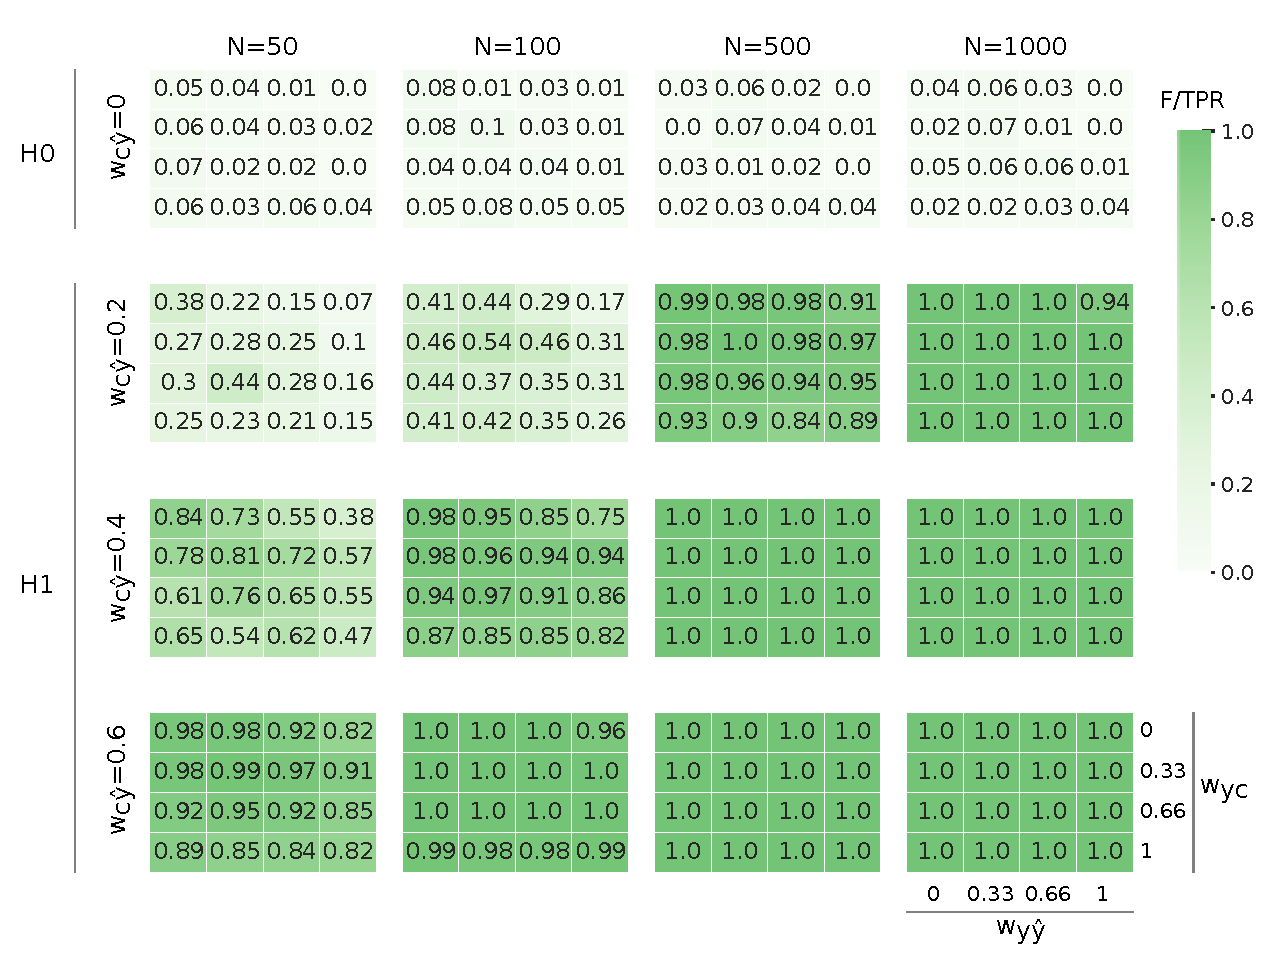
\includegraphics[width=0.75\paperwidth]{fig/sim_normal.eps}
  \caption{Simulation results.}
  \label{fig:hcp}
\end{figure}

\begin{figure}
  \centering
  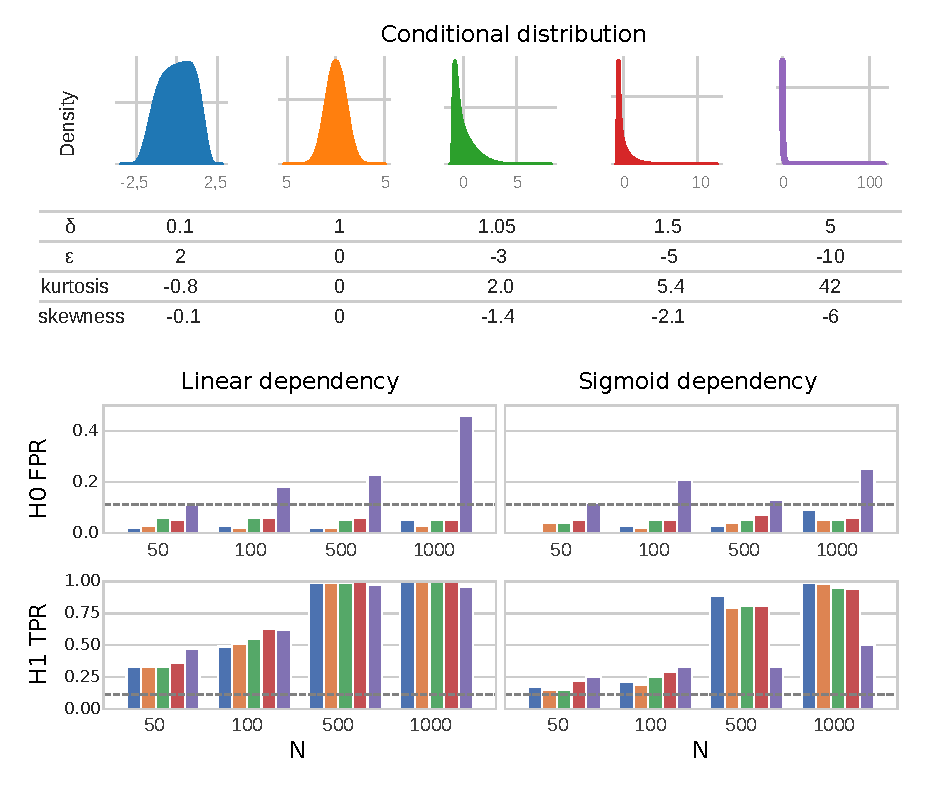
\includegraphics[width=0.50\paperwidth]{fig/sim_non-norm.eps}
  \caption{Simulation results, normality violation.}
  \label{fig:hcp}
\end{figure}

\subsection{Neuroimaging data}

\begin{figure}
  \centering
  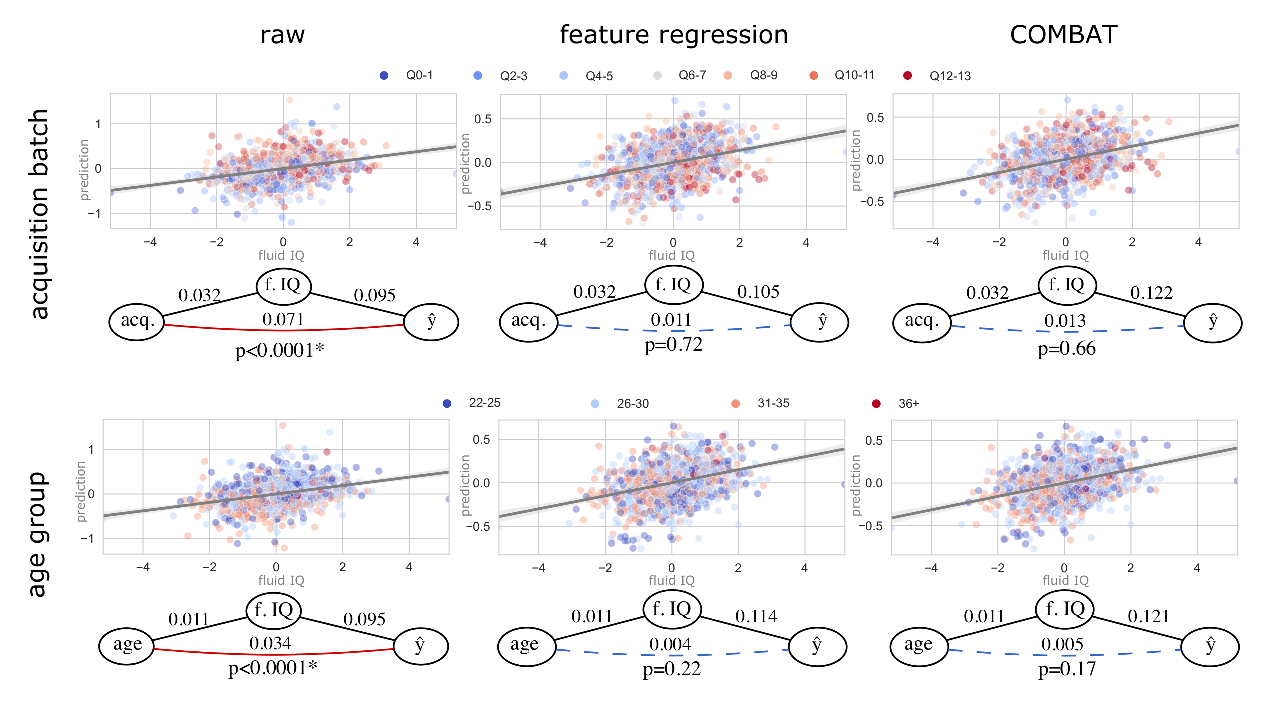
\includegraphics[width=0.75\paperwidth]{fig/fig_hcp.eps}
  \caption{Acquisition batch and age-bias of fluid IQ prediction in the HCP dataset.}
  \label{fig:hcp}
\end{figure}

\begin{figure}
  \centering
  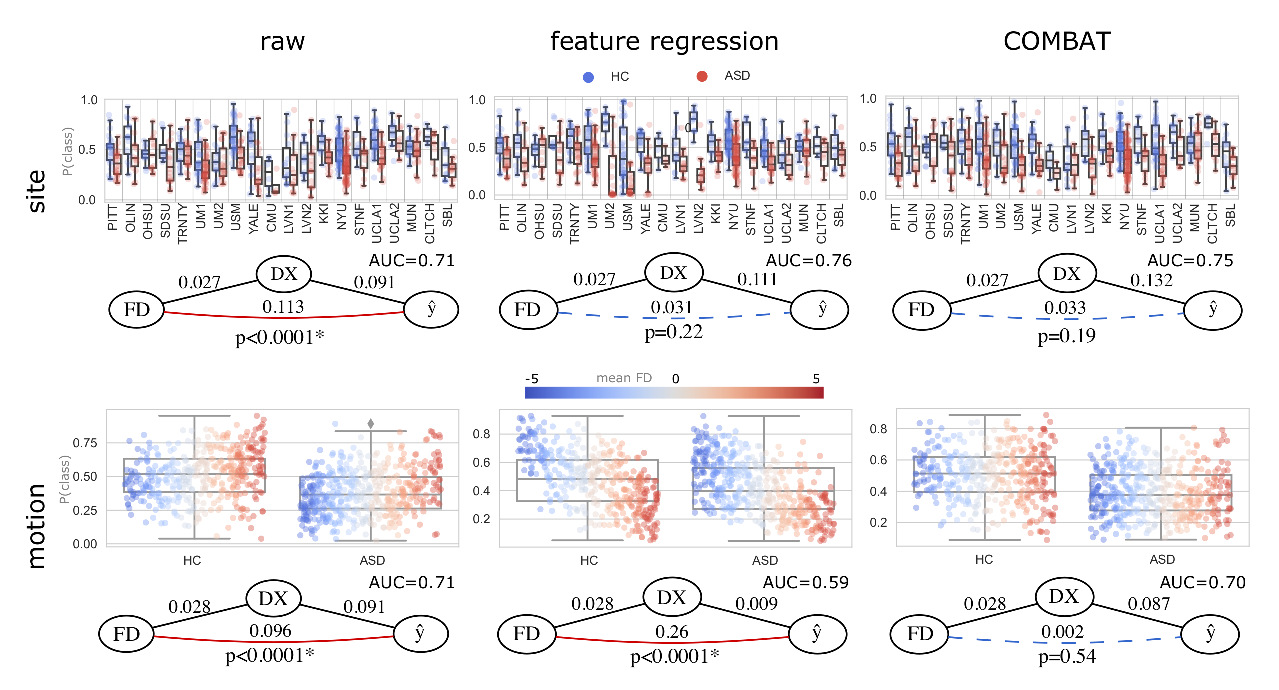
\includegraphics[width=0.75\paperwidth]{fig/fig_abide.eps}
  \caption{Center and motion-bias of ASD classification in the ABIDE dataset.}
  \label{fig:abide}
\end{figure}

%%%%%%%%%%%%%%%%%%%%%%%%%%%%%%%%%%%%%%%%%%%%%%%%%%%%%%%%%%%%%%%%%%%%%%%%%%%
\section{Discussion}

Applying predictive modelling and machine learning on functional neuroimaging data holds a great potential for both revolutionizing our understanding of the physical basis of mind and delivering clinically useful tools \citep{woo2017building, wager2013fmri, spisak2020pain}. However, the presence of confounders typical for biomedical research (e.g. demographics) and specific to the data acquisition and processing approach (e.g. imaging artifacts) present a great challenge to these efforts.

%%%%%%%%%%%%%%%%%%%%%%%%%%%%%%%%%%%%%%%%%%%%%%%%%%%%%%%%%%%%%%%%%%%%%%%%%%%
\section{Conclusion}


\bibliographystyle{apalike}  
\bibliography{references}

\newpage
\section{Supplementary Material}
\beginsupplement

\begin{figure}[H]
  \centering
  \fbox{
   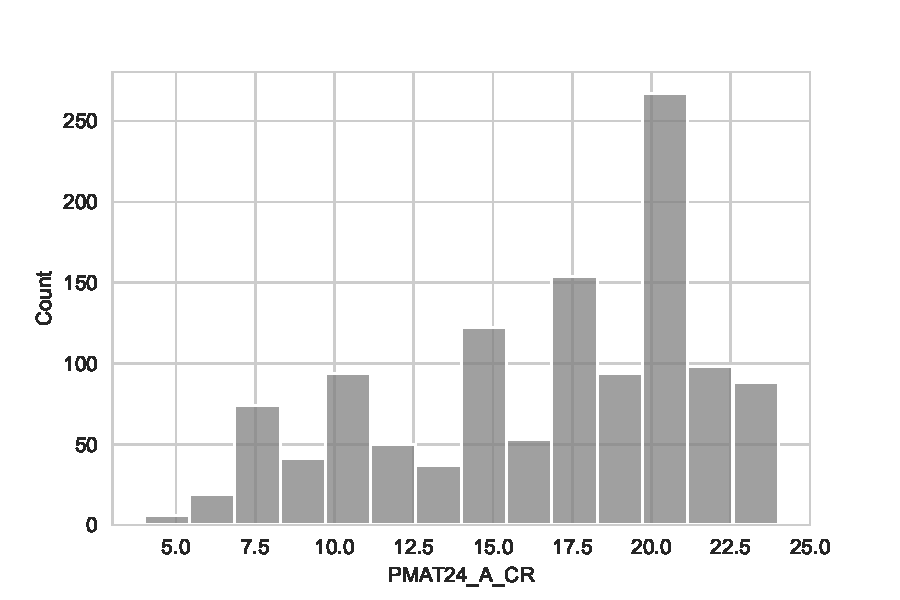
\includegraphics[width=0.36\paperwidth]{fig/hcp_iq_nonnorm_hist.pdf}
   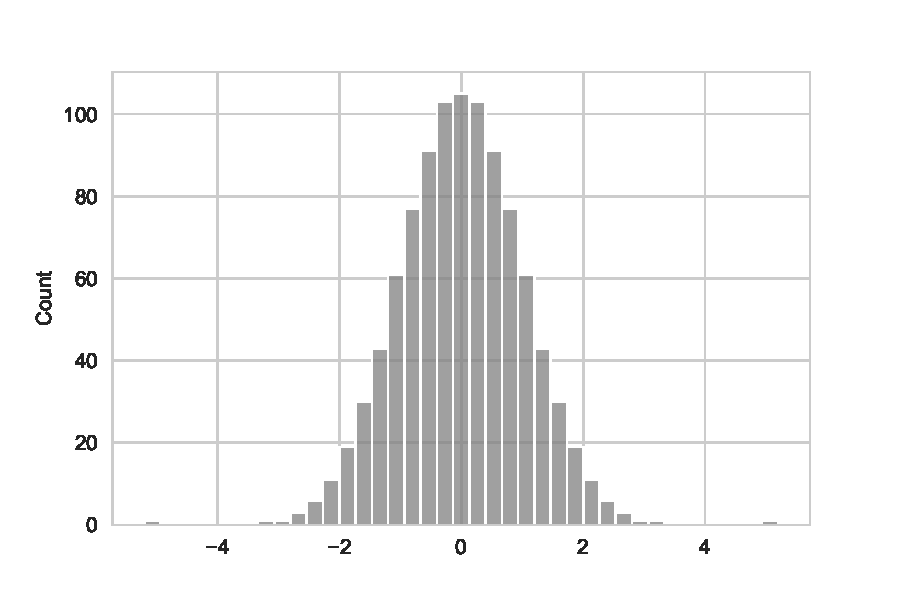
\includegraphics[width=0.36\paperwidth]{fig/hcp_iq_quanttrf_hist.pdf}
   }
  \caption{Histogram of fluid intelligence score in the HPC dataset, before (left) and after (right) quantile transformation.}
  \label{fig:hcp-hist}
\end{figure}

\begin{figure}[H]
  \centering
  \fbox{
   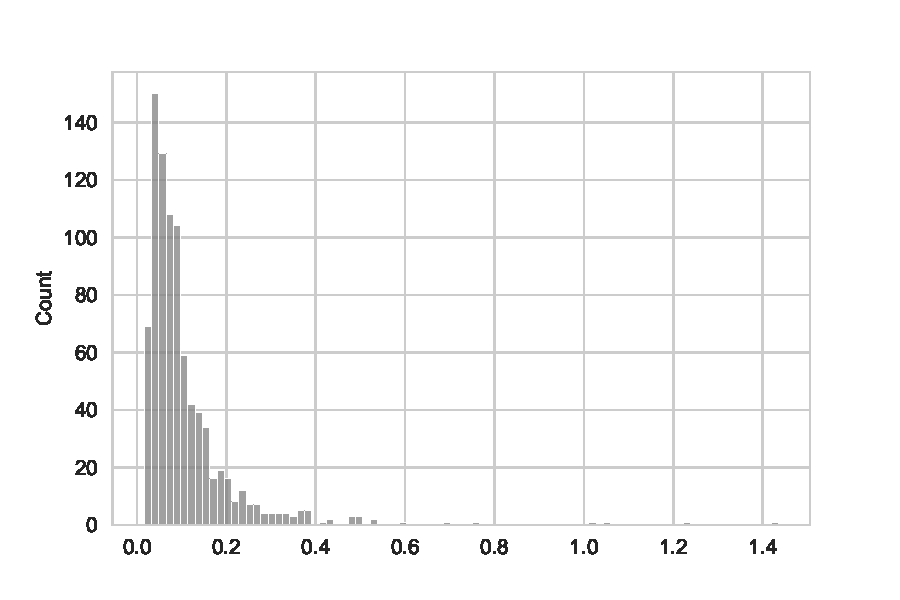
\includegraphics[width=0.36\paperwidth]{fig/abide_motion_hist.pdf}
   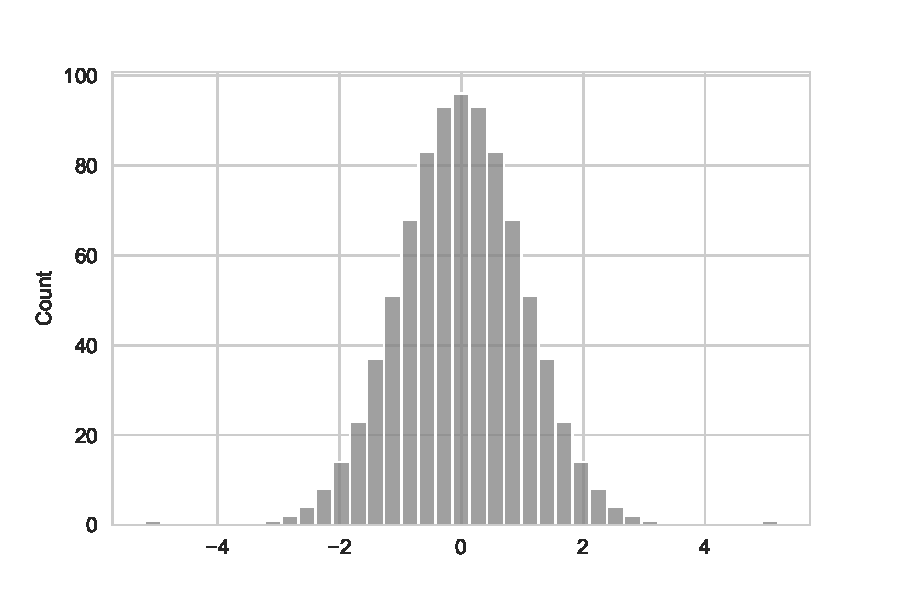
\includegraphics[width=0.36\paperwidth]{fig/abide_motion_quanttrf_hist.pdf}
   }
  \caption{Histogram of mean framewise displacement in the ABIDE dataset, before (left) and after (right) quantile transformation.}
  \label{fig:abide-hist}
\end{figure}


\end{document}
